% !TEX TS-program = XeLaTeX
% !TEX encoding = UTF-8 Unicode

\chapter{列表,三线表,插图,参考文献}
\label{chap02}

\section{列表}
\label{sec:23}

如果不是搞昆虫学,那就是连着几个月记着写那本大书《文化史上德谟克利特和柏拉
图两个流派》,或者是《形态学的发展》,或者是《应用生物学中的统计方法》,再不
然是他一九五一年至一九五二年编写的教程。几十、几百页都是这种枯燥无味、事
务性的记载,每天五至七行\footnote{格拉宁:《奇特的一生》页20}:
\begin{enumerate}
\item 鉴定袋蛾———二十分
\item 给斯拉瓦写信———二小时四十五分
\item 植物保护小组开会———二小时二十五分
\end{enumerate}

上述是默认的列表样式。源代码如下:
\begin{lstlisting}
  \begin{enumerate}
  \item 鉴定袋蛾———二十分
  \item 给斯拉瓦写信———二小时四十五分
  \item 植物保护小组开会———二小时二十五分
  \end{enumerate}
\end{lstlisting}

\texttt{emumerate}环境就是列表环境。每条\texttt{\textbackslash{item}}后面
跟一个空格,然后就是具体的条目。

默认的样式是按照(1),(2),(3)来排序的,如果想按照英文字母(a),(b),(c)或者罗
马数字(i),(ii),(iii)这样的顺序呢,只需要
在\texttt{\textbackslash{begin}\{enumerate\}}后面加一个参数,参数放在方括
号内。比如:
\begin{enumerate}[(a)]
\item 鉴定袋蛾———二十分
\item 给斯拉瓦写信———二小时四十五分
\item 植物保护小组开会———二小时二十五分
\end{enumerate}
源代码是:
\begin{lstlisting}
  \begin{enumerate}[(a)]
  \item 鉴定袋蛾———二十分
  \item 给斯拉瓦写信———二小时四十五分
  \item 植物保护小组开会———二小时二十五分
  \end{enumerate}
\end{lstlisting}

如上,方括号的中参数是可以更改的。a代表小写字母,A代表大写字母,1代表数
字,i代表小写罗马数字,I代表大写罗马数字。这些参数可以加上圆括号,也可以
加上一个点(英文句号)。\textcolor{red}{[a)]}:列表的标签就会变
成a)、b)、c)。\textcolor{red}{[1.]}:列表的标签就会变成1.、2.、3. 。

罗马数字的例子:
\begin{enumerate}[i.]
\item 鉴定袋蛾———二十分
\item 给斯拉瓦写信———二小时四十五分
\item 植物保护小组开会———二小时二十五分
\end{enumerate}
源代码:
\begin{lstlisting}
  \begin{enumerate}[i.]
  \item 鉴定袋蛾———二十分
  \item 给斯拉瓦写信———二小时四十五分
  \item 植物保护小组开会———二小时二十五分
  \end{enumerate}
\end{lstlisting}

\section{表}

\subsection{三线表}

\begin{figure}[htbp]
  \centering
  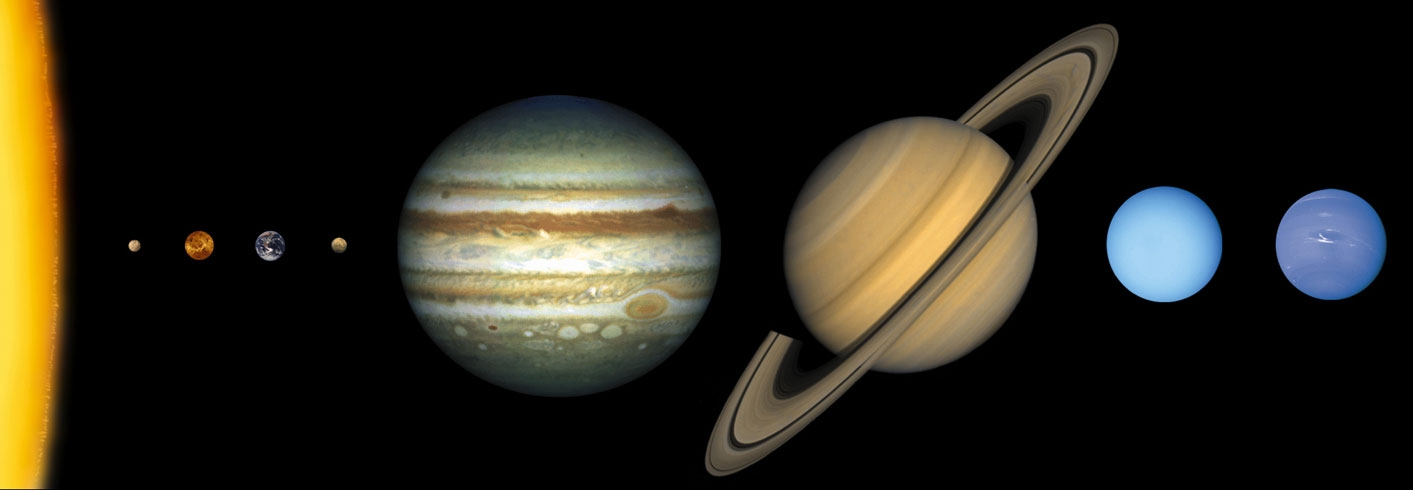
\includegraphics[width=0.9\textwidth{},keepaspectratio]{sun.jpg}
  \bicaption[fig:sun]{图}{最左侧是太阳,向右依序为水星、金星、地球、火星、
    木星、土星、天王星与海王星}{Fig.}{Outward from the Sun, the planets
    are Mercury, Venus, Earth, Mars, Jupiter, Saturn, Uranus and
    Neptune.}
\end{figure}

天文学家在太阳系内以天文单位(AU)来测量距离。1AU是地球到太阳的平均距离,
大约是\num{149598000}公里(\num{93000000}英里)。冥王星与太阳的距离大约
是39AU,木星则约是5.2AU。最常用在测量恒星距离的长度单位是光年,1光年大约
相当于\num{63240}天文单位\footnote{维基百科:太阳系}。

图~\ref{fig:sun}展示了太阳系的各行星的位置。

\begin{table}[htbp]
  \bicaption[tab:xingxing]{表}{行星数据表}{Tab.}{Planet}
  \centering
  \vspace{0.2cm}
  \zhongwu
  \begin{tabular}{cccc}
    \toprule
    Planet  & Size(Earth=1) & Weight(Earth=1) & Radius  \\
    \midrule
    Mercury & 0.056         & 0.055           & 0.3871  \\
    Venus   & 0.857         & 0.815           & 0.7233  \\
    Earth   & 1.00          & 1.000           & 1.0000  \\
    Mars    & 0.151         & 0.107           & 1.5237  \\ 
    Jupiter & 1321          & 317.832         & 5.2026  \\ 
    Saturn  & 755           & 95.16           & 9.5549  \\ 
    Uranus  & 63            & 14.54           & 19.2184 \\ 
    Neptune & 58            & 17.15           & 30.1104 \\ 
    \bottomrule
  \end{tabular}
\end{table}

表~\ref{tab:xingxing}就是最简单的三线表。源代码如下:
\begin{lstlisting}
  \begin{table}[htbp]
    \bicaption[tab:xingxing]{ 表 }{ 行星数据表 }{Tab.}{Planet}
    \centering
    \vspace{0.2cm}
    \zhongwu
    \begin{tabular}{cccc}
      \toprule
      Planet  & Size(Earth=1) & Weight(Earth=1) & Radius  \\
      \midrule
      Mercury & 0.056         & 0.055           & 0.3871  \\
      Venus   & 0.857         & 0.815           & 0.7233  \\ 
      Earth   & 1.00          & 1.000           & 1.0000  \\ 
      Mars    & 0.151         & 0.107           & 1.5237  \\ 
      Jupiter & 1321          & 317.832         & 5.2026  \\ 
      Saturn  & 755           & 95.16           & 9.5549  \\ 
      Uranus  & 63            & 14.54           & 19.2184 \\ 
      Neptune & 58            & 17.15           & 30.1104 \\
      \bottomrule
    \end{tabular}
  \end{table}
\end{lstlisting}


表格和插图通常需要占据大块空间,所以在文字处理软件中用户经常需要调整它们的
位置。\texttt{table}环境可以自动完成这样的任务;这种自动调整位置的环境称作
浮动环境 (float),下一节里还会介绍插图浮动环境\footnote{包太雷:\LaTeX{}
  NOTES———雷太赫排版系统简介}。

\texttt{htbp} 选项用来指定表格的理想位置,这几个字母分别代表 here, top,
bottom,float page,也就是就这里、页顶、页尾、浮动页 (专门放浮动环境的单独
页面)。我们可以使用这几个字母的任意组合,四个字母都写上表示放哪里都无所
谓;一般不推荐单独使用h,因为\LaTeX{}自以为它的排版算法是最完美的,不愿意
被束缚手脚。

\texttt{\textbackslash{centering}} 用来使表格居
中;\texttt{\textbackslash{bicaption}} 命令设置表格标题,\LaTeX{}会自动给
浮动环境的标题加上编号。

它的官方使用说明为:
\begin{lstlisting}
  \bicaption[label]{ 中文短标题 }{ 中文标题 }{Tab.}{ 英文标题 }
\end{lstlisting}
可选参数~\texttt{\footnotesize label}~用来作为交叉引用链接。例如
表~\ref{tab:xingxing}中的\texttt{lable}为\texttt{tab:xingxing}。这里的标
签一般为英文。中文短标题一般没什么用,可以随意填。最简单就是“表”。

在表格环境中,标题必须位于表格的上方。而在图片环境中,标题的位置必须位于
图片的下方。

\texttt{tabular} 环境提供了最简单的表格功能。它用 \texttt{\&} 来分列,
用 \texttt{\textbackslash{\textbackslash{}}} 来换行;每列可以采用居中、居
左、居右等横向对齐方式,分别用 \texttt{l、c、r} 来表示。

三线表的三条横线就分别
用 \texttt{\textbackslash{toprule}}、\texttt{\textbackslash{midrule}}、
\texttt{\textbackslash{bottomrule}} 等命令表示。

\texttt{\textbackslash{vspace}\{0.2cm\}}是用来控制表格标题与表格正文的
垂直间距的,请在插入表格时务必添加。\texttt{\textbackslash{zhongwu}}是
用来调整表格内容的行距的。


\subsection{表格的列按小数点对齐}

以表~\ref{tab:xingxing}为例,想把其中的第三列按小数点对齐\footnote{参见宏
  包siunitx}。先看一下效果:

在表~\ref{tab:xiaoshu}中,我们调整了原来四列数的对齐方式。原来
是\texttt{cccc},现在是\texttt{lcSr}。第一列左对齐,第二列不变,还是居中
对齐,第四列右对齐。值得注意的是第三列,这里新引入了一个参数\texttt{S},
含义就是这一列的数字按照小数点对齐。一定是大写的S。另外,第三列的列
头Weight(Earth=1)两边也加上了大括号,因为这不是数字。在使用参
数\texttt{S}的时候,不是数字的行需要用大括号括起来,不然会造成编译错误。

\begin{table}[htbp]
  \bicaption[tab:xiaoshu]{表}{行星数据表}{Tab.}{Planet}
  \centering
  \vspace{0.2cm}
  \zhongwu
  \begin{tabular}{lcSr}
    \toprule
    Planet  & Size(Earth=1) & {Weight(Earth=1)} & Radius  \\
    \midrule
    Mercury & 0.056         & 0.055           & 0.3871  \\
    Venus   & 0.857         & 0.815           & 0.7233  \\ 
    Earth   & 1.00          & 1.000           & 1.0000  \\ 
    Mars    & 0.151         & 0.107           & 1.5237  \\ 
    Jupiter & 1321          & 317.832         & 5.2026  \\ 
    Saturn  & 755           & 95.16           & 9.5549  \\ 
    Uranus  & 63            & 14.54           & 19.2184 \\ 
    Neptune & 58            & 17.15           & 30.1104 \\ 
    \bottomrule
  \end{tabular}
\end{table}

\begin{lstlisting}
  \begin{table}[htbp]
    \bicaption[tab:xiaoshu]{ 表 }{ 行星数据表 }{Tab.}{Planet}
    \centering
    \vspace{0.2cm}
    \zhongwu
    \begin{tabular}{lcSr}
      \toprule
      Planet  & Size(Earth=1) & {Weight(Earth=1)} & Radius  \\
      \midrule
      Mercury & 0.056         & 0.055           & 0.3871  \\
      Venus   & 0.857         & 0.815           & 0.7233  \\ 
      Earth   & 1.00          & 1.000           & 1.0000  \\ 
      Mars    & 0.151         & 0.107           & 1.5237  \\ 
      Jupiter & 1321          & 317.832         & 5.2026  \\ 
      Saturn  & 755           & 95.16           & 9.5549  \\ 
      Uranus  & 63            & 14.54           & 19.2184 \\ 
      Neptune & 58            & 17.15           & 30.1104 \\ 
      \bottomrule
    \end{tabular}
  \end{table}
\end{lstlisting}

\subsection{多列三线表}

在三线表中,有些列的列头会横跨好几列的数据。一般使
用\texttt{multicolumn}命令。它的用法是:
\begin{lstlisting}
  \multicolumn{ 列数}{ 对齐方式 }{ 表格内容 }
\end{lstlisting}

“列数”是指这一列横跨的列数,在表~\ref{tab:linux}是2列,就填“2”;“对
齐方式”从\texttt{lcr}三者中选其一即可,在表~\ref{tab:linux}中是c。“表格
内容”填入自己的内容。一般还会在这一列的下面画一小横线,已示辨识。使
用\texttt{cmidrule}命令。在表~\ref{tab:linux}中,由于横跨的是第2列和第3列,
因此\texttt{cmidrule}的参数是2-3。

\begin{table}[htbp]
  \bicaption[tab:linux]{}{ 不同操作系统下的\LaTeX{} }{Tab.}{OS with \LaTeX{}}
  \centering
  \vspace{0.2cm}
  \zhongwu
  \begin{tabular}{ccc}
    \toprule
    Test    & \multicolumn{2}{c}{Common Tools} \\
    \cmidrule{2-3}
    OS         & Distribution & Editor            \\
    \midrule
    Windows    & MikTeX       & TexMakerX         \\
    Mac OS     & MacTeX       & TeXShop           \\
    Linux/Unix & TeX Live     & TeXworks          \\
    \bottomrule
  \end{tabular}
\end{table}


\begin{lstlisting}
  \begin{table}[htbp]
    \bicaption[tab:linux]{}{ 不同操作系统下的\LaTeX{}}{Tab.}{OS with \LaTeX{}}
    \centering
    \vspace{0.2cm}
    \zhongwu
    \begin{tabular}{ccc}
      \toprule
      Test    & \multicolumn{2}{c}{Common Tools} \\
      \cmidrule{2-3}
      OS         & Distribution & Editor            \\
      \midrule
      Windows    & MikTeX       & TexMakerX         \\
      Mac OS     & MacTeX       & TeXShop           \\
      Linux/Unix & TeX Live     & TeXworks          \\
      \bottomrule
    \end{tabular}
  \end{table}
\end{lstlisting}

\subsection{多行三线表}

既然有多列三线表,多行三线表也是用类似的方法解决。我们把表~\ref{tab:linux} 来改造一下,相对应的,一般使用\texttt{multirow}命令。它的用法
是:
\begin{lstlisting}
  \multirow{ 行数 }*{ 表格内容 }
\end{lstlisting}

“行数”是指竖向跨的行数,在表~\ref{tab:unix}中是2行,中间有个星号,表示自然宽度。

\begin{table}[htbp]
  \bicaption[tab:unix]{}{ 不同操作系统下的\LaTeX{} }{Tab.}{OS with \LaTeX{}}
  \centering
  \vspace{0.2cm}
  \zhongwu
  \begin{tabular}{ccc}
    \toprule
    \multirow{2}*{OS} & \multicolumn{2}{c}{Common Tools} \\
    \cmidrule{2-3}
    & Distribution & Editor            \\
    \midrule
    Windows          & MikTeX       & TexMakerX         \\
    Mac OS           & MacTeX       & TeXShop           \\
    Linux/Unix       & TeX Live     & TeXworks          \\
    \bottomrule
  \end{tabular}
\end{table}


\begin{lstlisting}
  \begin{table}[htbp]
    \bicaption[tab:unix]{}{ 不同操作系统下的\LaTeX{} }{Tab.}{OS with \LaTeX{}}
    \centering
    \vspace{0.2cm}
    \zhongwu
    \begin{tabular}{ccc}
      \toprule
      \multirow{2}*{OS} & \multicolumn{2}{c}{Common Tools} \\
      \cmidrule{2-3}
      & Distribution & Editor            \\
      \midrule
      Windows          & MikTeX       & TexMakerX         \\
      Mac OS           & MacTeX       & TeXShop           \\
      Linux/Unix       & TeX Live     & TeXworks          \\
      \bottomrule
    \end{tabular}
  \end{table}
\end{lstlisting}

\subsection{宽度控制}

有时候表格中的某行太长了,需要折行。可以使用\texttt{tabularx} 宏包的同名
环境,其语法如下:

\begin{lstlisting}
  \begin{tabularx}{ 表格总宽度 }{ 对齐方式 }
    ...
  \end{tabularx}
\end{lstlisting}

“表格总宽度”最好用\texttt{textwidth}乘以某个系数表示。例
如\texttt{0.8\textbackslash{textwidth}}表示表格宽度是版芯宽度的0.8倍。这
样出来的效果比较好看。对齐方式除了原有的\texttt{l,c,r}之外,多了一
个\texttt{X},表示某列可以折行。

\begin{table}[htbp]
  \centering
  \bicaption[tab:wall]{ 表 }{ 墙上的44句话 }{Tab.}{Mikko Kuorinki}
  \vspace{0.2cm}
  \zhongwu
  \begin{tabularx}{0.8\textwidth{}}{lX}
    \toprule
    People & Says \\
    \midrule
    Elias Canetti & If you were alone, you would cut yourself in two, so
    that one part would shape the other.\\
    Franz Kafka & In the struggle between yourself and the world,
    second the world.\\
    \bottomrule
  \end{tabularx}
\end{table}

\begin{lstlisting}
  \begin{table}[htbp]
    \centering
    \bicaption[tab:figure]{ 表 }{ 墙上的44句话 }{Tab.}{Mikko Kuorinki}
    \vspace{0.2cm}
    \zhongwu
    \begin{tabularx}{0.8\textwidth{}}{lX}
      \toprule
      People & Says \\
      \midrule Elias Canetti & If you were alone, you would cut yourself
      in two, so  that one part would shape the other.\\
      Franz Kafka & In the struggle between yourself and the world,
      second the world.\\
      \bottomrule
    \end{tabularx}
  \end{table}
\end{lstlisting}



\subsection{斜线表头}

还是有些童鞋的表示三线表不实用啊,非要回归到原来的斜线表头去。我们可以使
用宏包\texttt{diagbox}提供的命令轻松完成。不过呢,出来的表格很ugly罢了。

\texttt{diagbox}是宏包提供的主要命令。它可以带有两个必选参数,表示要生成斜
线表头的两部分内容。默认斜线是从西北到东南方向的。

需要注意的是,使用斜线表格后就不能使用三线表的三条横线,不然请看
表~\ref{tab:diagbox}的下场。正确的做法是使用最原始的\texttt{hline},见
表~\ref{tab:xiexian}。

\begin{table}[htbp]
  \bicaption[tab:diagbox]{表}{斜线表头}{Tab.}{Diagbox}
  \centering
  \vspace{0.2cm}
  \zhongwu
  \begin{tabular}{|l|ccc|}
    \toprule
    \diagbox{Times}{Day} & Mon  & Tue  & Wed  \\
    \midrule
    Morning              & used & used &      \\
    Afternoon            &      & used & used \\
    \bottomrule
  \end{tabular}
\end{table}

\begin{lstlisting}
  \begin{table}[htbp]
    \bicaption[tab:diagbox]{ 表 }{ 斜线表头 }{Tab.}{Diagbox}
    \centering
    \vspace{0.2cm}
    \zhongwu
    \begin{tabular}{|l|ccc|}
      \toprule
      \diagbox{Times}{Day} & Mon  & Tue  & Wed  \\
      \midrule
      Morning              & used & used &      \\
      Afternoon            &      & used & used \\
      \bottomrule
    \end{tabular}
  \end{table}
\end{lstlisting}

\begin{table}[htbp]
  \bicaption[tab:xiexian]{ 表 }{斜线表头}{Tab.}{Diagbox}
  \centering
  \vspace{0.2cm}
  \zhongwu
  \begin{tabular}{|l|ccc|}
    \hline
    \diagbox{Times}{Day} & Mon  & Tue  & Wed  \\
    \hline
    Morning              & used & used &      \\
    Afternoon            &      & used & used \\
    \hline
  \end{tabular}
\end{table}

\begin{lstlisting}
  \begin{table}[htbp]
    \bicaption[tab:xiexian]{ 表 }{ 斜线表头 }{Tab.}{Diagbox}
    \centering
    \vspace{0.2cm}
    \zhongwu
    \begin{tabular}{|l|ccc|}
      \hline
      \diagbox{Times}{Day} & Mon  & Tue  & Wed  \\
      \hline
      Morning              & used & used &      \\
      Afternoon            &      & used & used \\
      \hline
    \end{tabular}
  \end{table}
\end{lstlisting}


\section{图}
\label{chap02:figure}

我来北京十一年,上学,上班,也积累了不少同学同事,但我一次他们的婚礼都没
有参加过。刚毕业的时候这种邀请很多,好象是种翻天覆地日新月异的见证,不怕
那些同学们伤心,我也知道人家是真心邀请的,但我真觉得我没跟他们谁好到真有
必要参加那些婚礼,所以我就不去。这次黄总的婚礼通知的突然,但我却很想去见
证一下,我的罪恶太多,正好也让天主顺便宽恕宽恕我,沾沾喜气\footnote{蚌病
  生珠:阳光下的婚礼}。

我挺佩服黄总他们俩的,他们就真的仅仅在婚礼当天才拍所谓的“婚纱照”。我觉
得这样挺好。身为摄影部的美女,周围全是靠摄影吃饭的人,的确没必要出去花冤
枉钱就为了拍几张照片。

\begin{figure}[htbp]
  \centering
  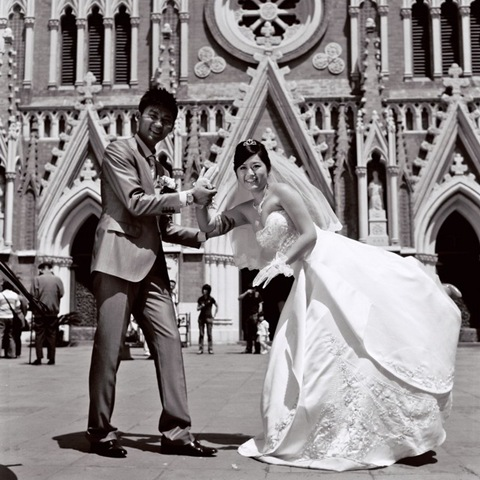
\includegraphics[scale=0.6]{wedding.jpg}
  \bicaption[fig:wedding]{婚礼}{婚礼}{Fig.}{Wedding}
\end{figure}

\begin{lstlisting}
  \begin{figure}[htbp]
    \centering
    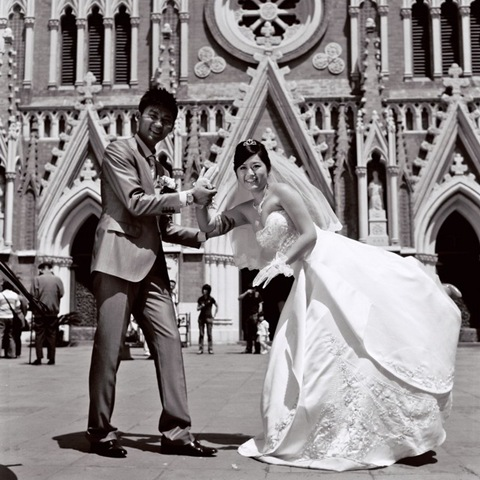
\includegraphics[scale=0.6]{wedding.jpg}
    \bicaption[fig:wedding]{ 婚礼 }{ 婚礼 }{Fig.}{Wedding}
  \end{figure}
\end{lstlisting}

论文使用的图片都放在figure文件夹中,插图浮动环境是\texttt{figure},基本命
令是\texttt{includegraphics},而在图片环境中,标题的位置必须位于图片的下
方。

\texttt{includegraphics}的基本参数见表~\ref{tab:figure}。

\begin{table}[htbp]
  \centering
  \bicaption[tab:figure]{插图命令参数}{插图命令参数}{Tab.}{Parameter}
  \vspace{0.2cm}
  \zhongwu
  \begin{tabularx}{0.8\textwidth{}}{lX}
    \toprule
    参数             & 说明 \\
    \midrule
    width=x,height=y & 宽度和高度,绝对尺寸,可用任意长度单位。                           \\
    scale=s          & 缩放比。绝对尺寸和缩放比用一种即可,同时使用两者,绝对尺寸起作用。 \\
    keepaspectratio & 保持图形比例。宽度和高度通常设置一个即可,否则图形比
    例会失调,除非再加上此选 项,
    这样图形宽度和高度都不超过指定参数。                                                \\
    angle=a          & 逆时针旋转角度,单位是度。                                        \\
    \bottomrule
  \end{tabularx}
\end{table}

对于图~\ref{fig:wedding},只使用了\texttt{scale}这一个参数,缩放因子是0.6。
当然,也可以直接指定图形的宽度和高度。图~\ref{fig:sun}的源代码如下:

\begin{lstlisting}
  \begin{figure}[htbp]
    \centering
    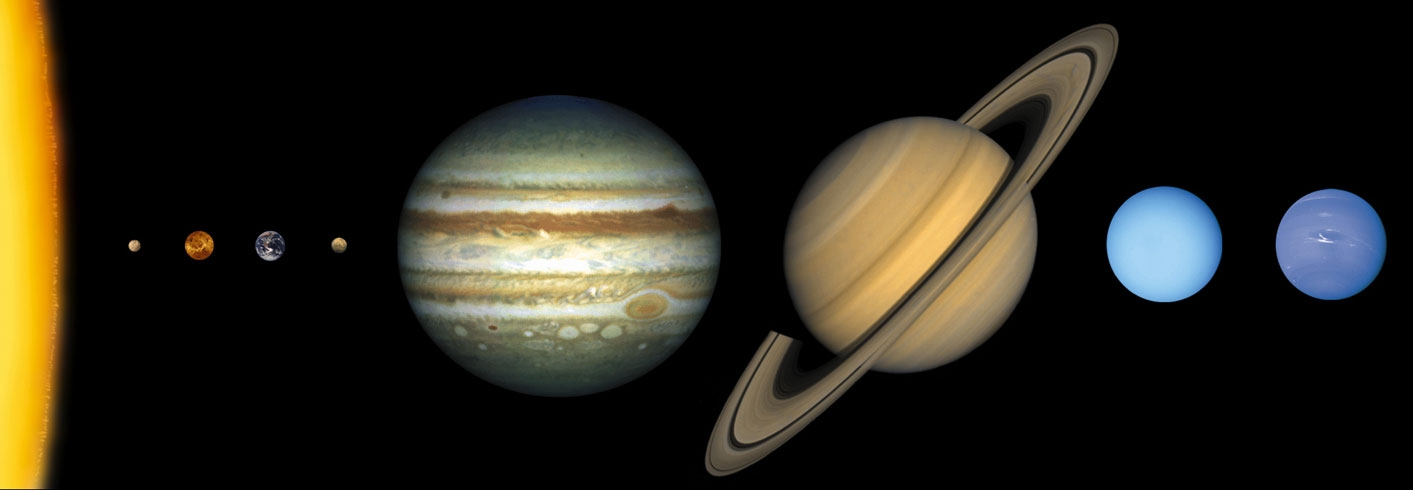
\includegraphics[width=\textwidth{},keepaspectratio]{sun.jpg}
    \bicaption[fig:sun]{ 图 }{ 最左侧是太阳,向右依序为水星、金
      星 }{Fig.}{Outward from the Sun, the planets are Mercury, Venus,
      Earth, Mars, Jupiter, Saturn, Uranus and Neptune.}
  \end{figure}
\end{lstlisting}

可以看到,图~\ref{fig:sun}的宽度指定为版芯的宽度,然后使用了保持宽高比这
个选项。


\subsection{双图并列}

温文敦厚的新郎,美丽可爱的新娘。

Alan和Cher这一对从校园时代就相偎相依一直到步入婚礼的殿堂。

我一直觉得,这样的情侣是最最难得的,两个人之间最珍贵的东西得以一直保存、
延续,直至在未来某个时候升华成为生命中不可名状的一种记忆和体验。这个世界
上有太多因为坚持或者不坚持,执着或者不执着导致的有始无终。能够沿路陪伴,
最终成为眷属,也算是不大不小的奇迹。

两个人的婚礼誓词很肉麻,很感人,写在小纸片上,认真的读出来,直到读到对方
流下感动的泪水,直到在场的嘉宾都用掌声回应这份真情\footnote{蚌病生珠:罗
  兰湖畔}。

\begin{figure}[htbp]
  \centering
  \begin{minipage}{0.4\textwidth}
    \centering
    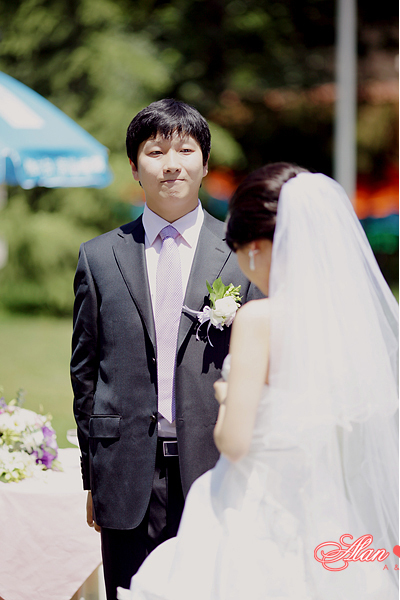
\includegraphics[keepaspectratio]{lang.jpg}
    \bicaption[fig:lang]{图}{新郎}{Fig.}{Bridegroom}
  \end{minipage}
  \begin{minipage}{0.4\textwidth}
    \centering
    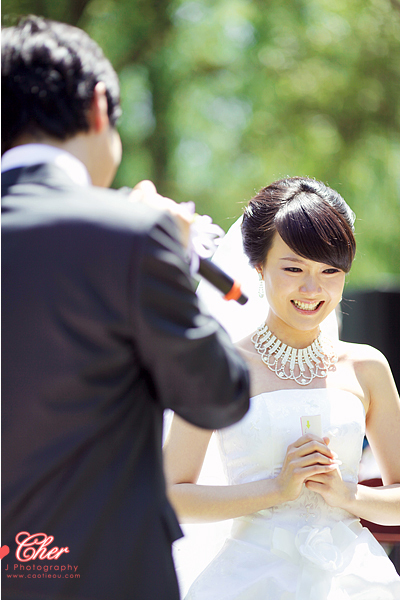
\includegraphics[keepaspectratio]{liang.jpg}
    \bicaption[fig:niang]{图}{新娘}{Fig.}{Brige}
  \end{minipage}
\end{figure}

\begin{lstlisting}
  \begin{figure}[htbp]
    \centering
    \begin{minipage}{0.4\textwidth}
      \centering
      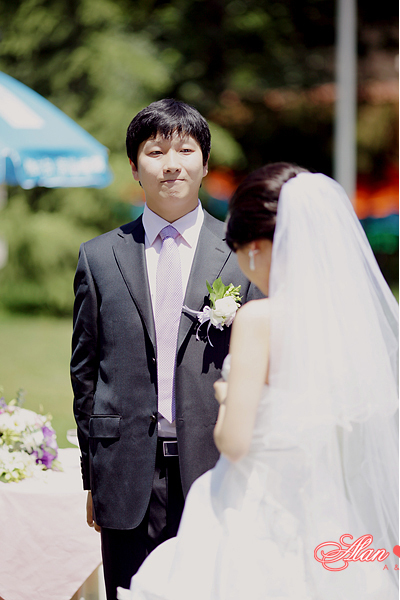
\includegraphics[keepaspectratio]{lang.jpg}
      \bicaption[fig:lang]{ 图 }{ 新郎 }{Fig.}{Bridegroom}
    \end{minipage}
    \begin{minipage}{0.4\textwidth}
      \centering
      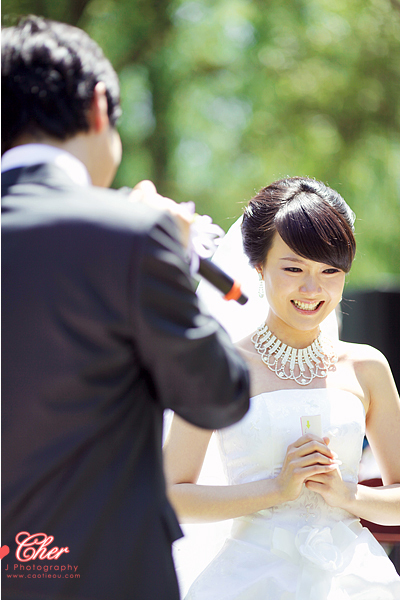
\includegraphics[keepaspectratio]{liang.jpg}
      \bicaption[fig:niang]{ 图}{ 新娘 }{Fig.}{Brige}
    \end{minipage}
  \end{figure}
\end{lstlisting}


如果想要两幅并排的插图各有自己的标题,可以在 figure 环境中使用两
个 \texttt{minipage} 环境,每个里面插入一幅图 (见图~\ref{fig:lang}和
图~\ref{fig:niang}) 。不用 \texttt{minipage} 的话,因为插图标题的缺省宽度是
整个行宽;两幅插图就会上下排列。

这里指定了每个\texttt{minipage}的宽度为0.4倍的版芯宽度。当然,也可以自
己指定,只是两个宽度加起来不超过版芯宽度就可以了。


\subsection{两子图并列}

有你在,开水瓶里永远都有水喝;冰箱里永远有一袋应急的速冻饺子;阳台的晾衣
架上我昨天换下的衣服已经有了今天太阳的味道;小猫也不用害怕得病和不舒服,
它们有最负责任的家庭医生;还有别人根本见都没见过的那些点心和饼干;还有,
你是我见过的少有的照片和本人都好看的女孩\footnote{蚌病生珠:Two-year
  anniversary}。


\begin{figure}[htbp]
  \centering
  \subfigure[超人A]{
    \label{fig:1a}
    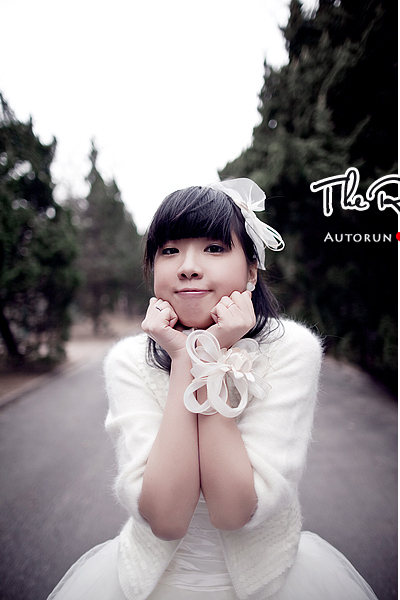
\includegraphics[keepaspectratio]{chao.jpg}
  }
  \hspace{20pt}
  \subfigure[超人A]{
    \label{fig:1b}
    
\includegraphics[keepaspectratio]{ren.jpg}
  }
  \bicaption[fig:judy]{图}{小超人老师}{Fig.}{Judy}
\end{figure}

\begin{lstlisting}
  \begin{figure}[htbp]
    \centering
    \subfigure[超人A]{
      \label{fig:1a}
      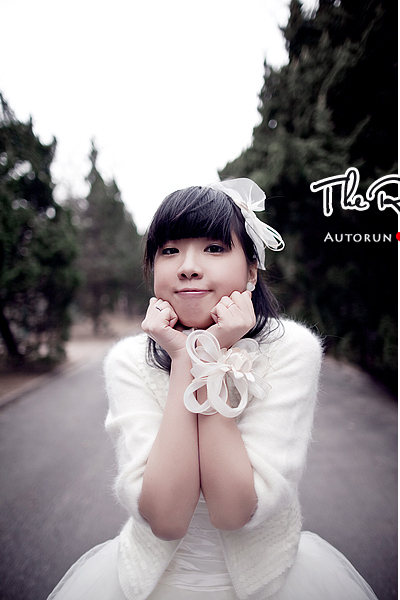
\includegraphics[keepaspectratio]{chao.jpg}
    }
    \hspace{20pt}
    \subfigure[超人A]{
      \label{fig:1b}
      
\includegraphics[keepaspectratio]{ren.jpg}
    }
    \bicaption[fig:judy]{图}{小超人老师}{Fig.}{Judy}
  \end{figure}
\end{lstlisting}

如果想要两幅并排的图片共享一个标题,并且各有自己的子标题,可以使
用\texttt{subcaption}宏包。如图~\ref{fig:judy},子图的标题用命令
\texttt{subcaption}即可。

\section{数学}

\subsection{math}

$\mathbf{A},\mathcal{A},\mathfrak{A},\mathbb{A}$

\begin{lstlisting}
  $\mathbf{A},\mathcal{A},\mathfrak{A},\mathbb{A}$
\end{lstlisting}

\subsection{傅立叶变换}

在现代数学中有一个很容易被外行误解的词汇:信号 (signal)。当数学家们说起
「一个信号」的时候,他们脑海中想到的并不是交通指示灯所发出的闪烁光芒或者
手机屏幕顶部的天线图案,而是一段可以具体数字化的信息,可以是声音,可以是
图像,也可是遥感测量数据。简单地说,它是一个函数,定义在通常的一维或者多
维空间之上。譬如一段声音就是一个定义在一维空间上的函数,自变量是时间,因
变量是声音的强度,一幅图像是定义在二维空间上的函数,自变量是横轴和纵轴坐
标,因变量是图像像素的色彩和明暗,如此等等\footnote{木遥:不确定性原理的
  前世今生 · 数学篇(一)}。

在数学上,关于一个信号最基本的问题在于如何将它表示和描述出来。按照上面所
说的办法,把一个信号理解成一个定义在时间或空间上的函数是一种自然而然的表
示方式,但是它对理解这一信号的内容来说常常不够。例如一段声音,如果单纯按
照定义在时间上的函数来表示,它画出来是这个样子的:

\begin{figure}[htbp]
  \centering
  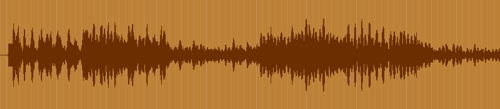
\includegraphics[width=0.8\textwidth{},keepaspectratio]{VisualAudio.png}
  \bicaption[fig:boxingtu]{波形图}{波形图}{Fig.}{Wave}
\end{figure}

图~\ref{fig:boxingtu}通常被称为波形图。毫无疑问,它包含了关于这段声音的全
部信息。但是同样毫无疑问的是,这些信息几乎没法从上面这个「函数」中直接看
出来,事实上,它只不过是巴赫的小提琴无伴奏 Partita No.3 的序曲开头几个小
节。图~\ref{fig:bahe} 是巴赫的手稿,从某种意义上说来,它也构成了对上面那
段声音的一个「描述」:

\begin{figure}[htbp]
  \centering
  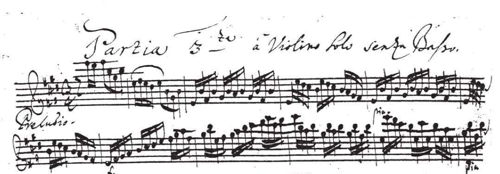
\includegraphics[width=0.8\textwidth{},keepaspectratio]{Partita3.png}
  \bicaption[fig:bahe]{巴赫手稿}{巴赫手稿}{Fig.}{Partita No.3}
\end{figure}

这两种描述之间的关系是怎样的呢?第一种描述刻划的是具体的信号数值,第二种
描述刻划的是声音的高低(即声音震动的频率)。人们直到十九世纪才渐渐意识到,
在这两种描述之间,事实上存在着一种对偶的关系,而这一点并不显然。

1807 年,法国数学家傅立叶 (J. Fourier) 提出了一个崭新的观念:任何一个函数
都可以表达为一系列不同频率的简谐振动(即简单的三角函数)的叠加。

用今天的语言来描述,傅立叶的发现实际上是在说:任何一个信号都可以用两种方
式来表达,一种就是通常意义上的表达,自变量是时间或者空间的坐标,因变量是
信号在该处的强度,另一种则是把一个信号「展开」成不同频率的简单三角函数
(简谐振动)的叠加,于是这就相当于把它看作是定义在所有频率所组成的空间
(称为频域空间)上的另一个函数,自变量是不同的频率,因变量是该频率所对应
的简谐振动的幅度。


这两个函数一个定义在时域(或空域)上,一个定义在频域上,看起来的样子通常
截然不同,但是它们是在以完全不同的方式殊途同归地描述着同一个信号。它们就
象是两种不同的语言,乍一听完全不相干,但是其实可以精确地互相翻译。在数学
上,这种翻译的过程被称为「傅立叶变换」。

傅立叶变换是一个数学上极为精美的对象:
\begin{enumerate}
\item 它是完全可逆的,任何能量有限的时域或空域信号都存在唯一的频域表达,
  反之亦然 。
\item 它完全不损伤信号的内在结构:任何两个信号之间有多少相关程度(即内
  积),它们的频域表达之间也一定有同样多的相关程度。
\item 它不改变信号之间的关联性:一组信号收敛到一个特定的极限,它们的频域
  表达也一定收敛到那个极限函数的频域表达。
\end{enumerate}

在傅立叶变换的所有这些数学性质中,最不寻常的是这样一种特性:一个在时域或
空域上看起来很复杂的信号(譬如一段声音或者一幅图像)通常在频域上的表达会
很简单。这里「简单」的意思是说作为频域上的函数,它只集中在很小一块区域内,
而很大一部分数值都接近于零。

一个在空域中看起来占满全空间的信号,从频域中看起来很可能只不过占用了极小
一块区域,而大部分频率是被浪费了的。这就导出了一个极为有用的结论:一个看
起来信息量很大的信号,其实可以只用少得多的数据来加以描述。只要对它先做傅
立叶变换,然后只记录那些不接近零的频域信息就可以了,这样数据量就可以大大
减少。

基本上,这正是今天大多数数据压缩方法的基础思想。在互联网时代,大量的多媒
体信息需要在尽量节省带宽和时间的前提下被传输,所以数据压缩从来都是最核心
的问题之一。而今天几乎所有流行的数据压缩格式,无论是声音的 mp3 格式还是图
像的 jpg 格式,都是利用傅立叶变换才得以发明的。从这个意义上说来,几乎全部
现代信息社会都建立在傅立叶的理论的基础之上。



\section{参考文献}


硕士论文写了3周。90多页英文,昏天黑地没日没夜写到想吐。好在有几个欧洲博士
后帮忙改语法错。改的他们也很想哭。后来已经功成名就论文无数ACM
Fellow英国Fellow of Royal Society的老板来给我们讲,写论文最重要的是
写Introduction。写Introduction就和写童话一样\footnote{珵cici:硕士论文你有
  哪些经验与收获?耗時多久?}。

\begin{enumerate}[1.]
\item 有一条巨龙抓走了公主 (介绍你的问题为什么值得研究)
\item 巨龙是多么多么多么难打(强调你的研究的重要性)
\item 王子提着一把金光闪闪的剑而不是破斧子烂长矛登场(你的方法好在哪里,别人sui在哪里)
\item 王子是如何打败巨龙(你的方法简介)
\item 从此王子和公主幸福的生活在一起。(解决了问题)
\end{enumerate}

老板说写论文就是写童话嘛。其余的也不过就是把这些东西细节讲一讲。做研究很
简单的。听完我就不想再做研究了。合着我写到吐血掉头发的时候大牛都把写论文
当给小盆友写童话。


我们的一切知识都是从经验开始\cite{李秋零1999},这是没有任何怀疑的\cite{邓晓芒2005}\cite{邓晓芒2000};
因为,如果不是对象激动我们的感官,一则由它们自己引起表象,一则使我们的知性活动运作起来,对这些表象加
以比较,把它们粘结或分开,\cite{欧进萍1999,欧进萍1991}这样把感性印象的原始素材加工成称之为经验的对象
知识,那么知识能力又该由什么来唤起活动呢?\cite{braun2007,kelton2002,strawderman2001,李秋零1999}所以
按照时间,我们没有任何知识是先行于经验的,一切知识都是从经验开始的。

只要是中文文献,图书,期刊,会议,专利等等需要为每个条目增加一个域:
\begin{lstlisting}
  language={c},
\end{lstlisting}

对于参考文献[1],原先的bib文件是这样的:
\begin{lstlisting}
  @article{ 李秋零1999 ,
    title={ 康德何以步安瑟尔谟的后尘? },
    author={ 李秋零 },
    journal={ 中国人民大学学报 },
    volume={2},
    year={1999}
  }
\end{lstlisting}


但是由于是中文文献,需要增加一个语言域,就变成下列样式:
\begin{lstlisting}
  @article{ 李秋零1999,
    title={ 康德何以步安瑟尔谟的后尘? },
    author={ 李秋零 },
    language={c},
    journal={ 中国人民大学学报 },
    volume={2},
    year={1999}
  }
\end{lstlisting}
